% !TEX encoding = UTF-8 Unicode
\documentclass[12pt,oneside]{fithesis2}
\usepackage[english]{babel}       % Multilingual support
\usepackage[utf8]{inputenc}       % UTF-8 encoding
\usepackage[T1]{fontenc}          % T1 font encoding
\usepackage[                      % A sans serif font that blends well with Palatino
  scaled=0.86
]{berasans}
\usepackage[                      % A tt font if you do not like LM's tt
  scaled=1.03
]{inconsolata}
\usepackage[                      % Clickable links
  plainpages = false,               % We have multiple page numberings
  pdfpagelabels                     % Generate pdf page labels
]{hyperref}
\usepackage{blindtext}            % Lorem ipsum generator
\usepackage{graphicx}
\usepackage{svg}
\usepackage{amsmath}
\usepackage{hyperref}
\usepackage{tikz}
\usepackage{pgfplots}
\usepackage{pgfplotstable}
\usepackage{float}

\thesislang{en}                   % The language of the thesis
\thesistitle{Time Series Prediction Using Neural Networks}       % The title of the thesis
\thesissubtitle{Bachelor Thesis}  % The type of the thesis
\thesisstudent{Karol Kuna}          % Your name
\thesiswoman{false}                % Your gender
\thesisfaculty{fi}                % Your faculty
\thesisyear{Spring \the\year}     % The academic term of your thesis defense
\thesisadvisor{doc. RNDr. Tomáš Brázdil, Ph.D.}   % Your advisor

%\DeclareMathSizes{14}{14}{8}{8} %display/text style, script style and scriptscript style.

\begin{document}
  \FrontMatter                    % The front matter
    \ThesisTitlePage                % The title page
    \begin{ThesisDeclaration}       % The declaration
      \DeclarationText
      \AdvisorName
    \end{ThesisDeclaration}
    \begin{ThesisThanks}            % The acknowledgements (optional)
      I would like to thank my advisor, Tomáš Brázdil for all the help and guidance he has provided.
    \end{ThesisThanks}
    \begin{ThesisAbstract}          % The abstract
      This thesis compares existing methods for predicting time series in real time using neural networks. Focus is put on recurrent neural networks (RNNs) and online learning algorithms, such as Real-Time Recurrent Learning and truncated Backpropagation Through Time. In addition to the standard Elman's RNN architecture, \mbox{Clockwork-RNN} is examined. Methods are compared in terms of prediction accuracy and computation time, which is critical in real-time applications. Part of the work is experimental implementation of the tested models and working applications in robotics and  network traffic monitoring.
    \end{ThesisAbstract}
    \begin{ThesisKeyWords}          % The keywords
	time series, prediction, neural network, recurrent network, backpropagation, backpropagation through time, real-time recurrent learning, clockwork recurrent network
    \end{ThesisKeyWords}
    \tableofcontents                % The table of contents
   \listoftables                   % The list of tables (optional)
   \listoffigures                  % The list of figures (optional)
   
  
  \MainMatter
    \chapter{Introduction} %what is prediction and anomaly detection, why   
Each year more and more data is collected from high velocity data streams. Machine learning algorithms are used to analyse and create models of the data. Patterns found in the data structure are then exploited to make predictions about the future which can be used to guide decision making. In this thesis, I compare various artificial neural network (ANN) architectures and learning algorithms for online prediction of time series.

\par %neural networks, modelling data?
One of the most popular machine learning models are ANNs which are capable of approximating unknown functions and processes and thus are good candidates for use in prediction. Inspired by biological neural networks, ANNs consist of artificial neurons wired together to form a network.
\par %which networks are compared
Common neural network architectures, such as time delay neural networks (TDNNs) and simple recurrent networks (SRNs) trained by Truncated Backpropagation Through Time (TBPTT) and Real-Time Recurrent Learning (RTRL), as well as latest Clockwork RNN (CW-RNN) trained by TBPTT are evaluated in this thesis. Algorithms are compared in terms of prediction accuracy as well as computation time and the trade-off between them.
\par %what are time series
Time series are sequences of data points in time, usually created by measuring output of some process in discrete time intervals. The goal of prediction is to successfully estimate output of the process in next time step or several steps. It is assumed that the process is at least partially observable and to some extent, future values can be determined by observing past values. Prediction then reduces to problem of process approximation.
\par %describe the value of online prediction
Since value of stored data decreases over time, effort is put into gaining insight from data as they come. Many applications don't require storing data at all, or storing it would be impractical, therefore it is advantageous to create models and update them with every data point. Continuous online learning is well suited for such tasks and can adapt to changing environments without human intervention.
\par %applications described in this thesis, TODO: add citations. scenarios or applications?
Quality and speed of prediction is tested in one synthetic test and two application scenarios. The first scenario is robotic arm simulator implemented in 3D physics library BEPUPhysics. Manipulator with three actuated joints is created, the goal is to predict future position of robot's arm. The prediction network should act as a virtual model of the body, which can be useful in control systems.

%Data points that do not conform to the learned model of normal behaviour are called anomalies. Detecting anomalies is found to be increasingly important in computer network security. An anomaly may signal unexpected events, such as computer being under denial of service attack or unforeseen load.

\par %anomaly detection in network
The second scenario is monitoring utilisation of computer resources such as processor, memory, disk, and network usage. Neural networks should constantly predict future volume of incoming and outgoing network traffic and detect unexpected events called anomalies. When an unexpected computer network event occurs, it needs to be logged for an administrator to examine.
\par

\chapter{Prediction}
\section{Time Series}
Time series are sequences of data points measured over time. In this thesis, data points are real-valued vectors implemented as arrays of floating point numbers. \par
Data sequence is created by measuring output of a process at discrete, regular time intervals. Process may also receive input in every time step, which affects its future behaviour, or it may be purely generative receiving no input at all. For generalisation's sake, let's assume every process receives input which is a real-valued vector just like output. Generative processes then simply receive input vector of zero length.
	\begin{figure}[ht]
		\centering
		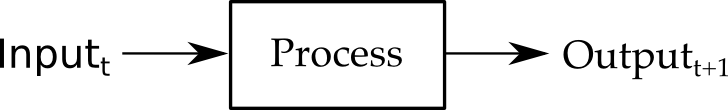
\includegraphics[width=182px]{process.png}
		\caption{Schema of a process.}
	\end{figure}
In every time step, process receives input, updates its internal state and produces output. Internal state of the process is usually hidden and can be observed only partially from output of the process. %any assumptions?

\section{Prediction}
The goal of prediction is to approximate the process as closely as possible and hence minimise forecast error, i.e. difference between actual and forecasted value \cite{timeseries}.\par
Naive approaches include methods like averaging past data points, returning previous data point or linear extrapolation. While these methods may suffice for some very simple time series, more sophisticated methods are required to cope with real-world time series. Sophisticated methods use historical data to estimate future value by finding a model of the process that empirically fits past data. \par
The problem of prediction can be alternatively viewed as problem of function approximation.
	$$\left(State_{t+1}, Output_{t+1}\right) = Process(State_t, Input_t)$$
Process is a function from current internal state and input to next internal state and output. Unfortunately, internal state is unknown, so next output can only be estimated from history of inputs and outputs. History can be defined as an ordered set of past inputs and outputs.
	$$History_t = \left( (Input_{t}, Output_{t}), \dots, (Input_{0}, Output_{0}) \right)$$
Prediction of the output in next time step is then a function from current history to next output.
	$$Output_{t+1} \approx Prediction_{1}( History_t )$$

\section{Prediction Horizon}
Some applications require estimating output of the process more than one step into the future. Prediction horizon is the number of time steps between current data point and the future predicted data point. Since future output of the process depends on inputs that will be fed in, these inputs have to be known beforehand. The modified $Prediction$ function of the process output $h$ steps in future is then
	$$Output_{t+h} \approx Prediction_{h}( History_t, (Input_{t+1}, \dots, Input_{t+h}) )$$

An alternative method for predicting multiple steps of the future is using one step prediction to estimate future process output, adding it to history as if it was actually measured together with the appropriate future input, and repeating this until prediction horizon is reached.

\chapter{Artificial Neural Networks}
Inspired by biological neural networks, ANNs are groups of elementary processing units called artificial neurons connected together to form a directed graph \cite{haykin2009neural}. Nodes of the graph represent biological neurons and connections between them represent synapses. Unlike in biological neural networks, connections between artificial neurons aren't usually added or removed after the network was created. Instead, connections are weighted and the weights are adapted by learning algorithm. \par

Input signal propagates through the network in the direction of connections until it reaches output of the network. In supervised learning, learning algorithm adapts the weights in order to minimise the difference between output of the network and desired output provided by teacher.

\section{Artificial Neuron}
The complex behaviour of biological neurons was simplified to create a mathematical model of artificial neurons, also called units. \par
Unit receives its inputs via input connections from other units' outputs, called activations. Then it calculates a weighted sum of the inputs, called potential. Finally, unit's activation is computed from the potential and sent to other units. \par

Weights of connections between units are stored in a matrix $w$, where $w_{ij}$ denotes weight of the connection from unit $i$ to unit $j$. Every unit $j$ has a potential $p_j$ which is calculated as weighted sum of all of its $N$ input units and bias. \par

$$p_{j} = \sum\limits_{i = 1}^{N+1} w_{ij} a_{i}$$

Bias term, also known as threshold unit, is usually represented as an extra input unit whose activation always equals one, therefore $a_{N+1} = 1$. Presence of bias term enables shifting the activation function along x-axis by changing the weight of connection from threshold unit.

Activation of the unit $a_j$ is then computed by transforming its potential $p_j$ by a non-linear activation function $act$.

$$a_{j} = act\left(p_j\right)$$
\par
Commonly used non-linear activation function ranging from 0 to 1 is sigmoid function thanks to its easily computable derivative which is used by learning algorithms.

$$\sigma(x) = {1 \over {1 + e^{-x}}}$$
$${{d\sigma(x)} \over dx} = \sigma(x)  \left(1 - \sigma(x)\right)$$

\section{Feedforward Neural Networks}
Feedforward neural networks are a subset of ANNs whose nodes form an acyclic graph where information moves only in one direction, from input to output. \par
Multilayer perceptron (MLP) is a class of feedforward networks consisting of three or more layers of units. Layer is a group of units receiving connections from the same units. Units inside a layer are not connected to each other. \par
	\begin{figure}[ht]
		\centering
		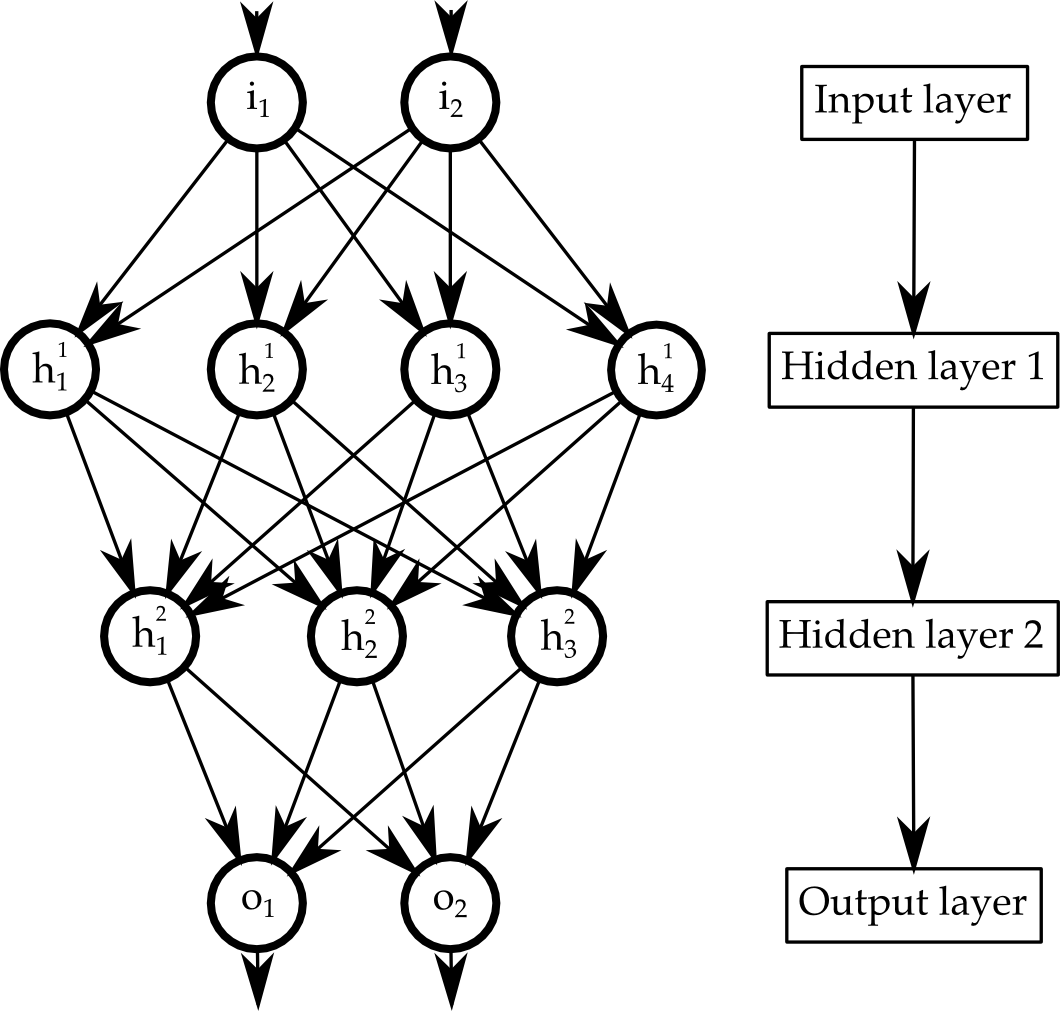
\includegraphics[width=265px]{mlp.png}
		\caption{On the left, MLP consisting of input layer with two units, two hidden layers with four and three units respectively, and output layer with two units. Schematic diagram of the MLP's layers on the right.}
	\end{figure}
MLP consists of three types of layers: input layer, one or more hidden layers and output layer. Input layer is the first layer of network and it receives no connections from other units, but instead holds network's input vector as activation of its units. Input layer is fully connected to first hidden layer. Hidden layer $i$ is then fully connected to hidden layer $i + 1$. Last hidden layer is fully connected to output layer. Activation of output units is considered to be output of the network. \par
The output of the network is calculated in a process called forward propagation in three steps :
\begin{enumerate}
	\item Network's input is copied to activations of input units
	\item Hidden layers compute their activations in topological order
	\item Output layer computes its activation and copies it to network's output
\end{enumerate}

MLPs are often used to approximate unknown functions from their inputs to outputs. MLP's capability of approximating any continuous function with support in the unit hypercube with only single hidden layer and sigmoid activation function was first proved by George Cybenko \cite{universal-approx-theorem}.

\subsection{Backpropagation}
\label{bp}
Backpropagation, or backward propagation of errors, is the most used supervised learning algorithm for adapting connection weights of feedforward ANNs. Weights of the network are tuned so as to minimise square error
$$E = {1 \over 2} \sum\limits_{i=1}^{N}(target_i - output_i)^2$$
where $target$ denotes desired output provided by teacher and $output$ is network's prediction of the output for the corresponding input, both of size $N$. \par
Considering error $E$ as a function of network's weights $w$, backpropagation can be seen as optimisation problem and standard gradient descent method can be applied. Local minimum is approached by changing weights along the direction of negative error gradient 
$$-{{\partial E} \over {\partial w}}$$
by weight change $\Delta w_{ij}$ proportionally to $\alpha$, which is constant positive value called learning rate. Fraction of previous weight change called momentum rate $\beta$ can be added to the current weight change, which often speeds up learning process \cite{sutskever}.
$$new \; \Delta w_{ij} = \beta \Delta w_{ij} - \alpha {{\partial E} \over {\partial w_{ij}}}$$
$$new \; w_{ij} = w_{ij} + \Delta w_{ij} $$


The central part of the algorithm is finding the error gradient. Let there be an MLP with $L$ layers in topological order, first being input and last being output layer. Layer $k$ has $U_k$ units and holds a weight matrix $w_{ij}^k$ representing weights of connections from unit $i$ in layer $k - 1$ to unit $j$ in layer $k$. Input layer has no incoming connections. The computation can be then divided into three steps:

\begin{enumerate}
  \item \textbf{Forward propagation}. Input vector is copied to activations $a_i^1$ of input layer units $i$. For every hidden or output layer $k$ in topological order, compute for every unit $i$ its potential (weighted input) $p_i^k$ and activation $a_i^k$.
  
  \item \textbf{Backward propagation}. Compute $\Delta^L_i$ i.e. the derivative of error $E$  w.r.t. activation $a_i^L$ of output layer unit $i$ as
  $$\Delta^L_i = \left(target_i - a^L_i\right){{\partial{act\left(p^L_i\right)}} \over {\partial p^L_i}}$$
 For hidden layer $h$ in reverse topological order starting from last hidden layer $h = L-1$ down to first input layer $h=2$ and its units $i$ compute error term as
 
  $$\Delta^h_i = \sum\limits_{j=1}^{U_{h + 1}} \Delta_{j}^{h+1}w_{ij}^{h+1} {{\partial{act\left(p^h_i\right)}} \over {\partial p^h_i}}$$
  
  \item \textbf{Weights update}. Change weights in layer $k$ according to
  $$new \; \Delta w_{ij}^k = \beta \Delta w_{ij}^k + \alpha \Delta_i^{k+1} a_{j}^{k}$$
  $$new \; w_{ij}^k = w_{ij}^k +  \Delta w_{ij}^k$$

\end{enumerate}

%conclusion about backprop

\subsection{Time-Delay Neural Networks}
Time-Delay Neural Network (TDNN) is a modification of feedforward network designed to capture dynamics of modelled process \cite{phoneme-recognition-tdnn}. As FFNs have no internal memory to store information about past, they are insufficient for processing temporal sequences. To overcome this, memory of past is introduced by means of extending network's input with sliding window of previous inputs, also known as tapped delay line. The information about the past is thus stored in the network input itself. Because there are no modifications to the network topology, standard backpropagation algorithm can be used.\par
Size of the sliding window determines how many past inputs are stored and consequently how much past data can be correlated to future output. Too small window may not capture necessary dynamics of the system, because network is blind to anything that happened before, and thus create inferior results. Whereas too large window can drastically prolong learning time.\par
To generalise TDNN to processes that also receive input, prediction of process output in next time step can be defined as approximation of function $Prediction_{TDNN}$ with window size $w$
	\[
		\begin{split}
		Output_{t+1} \approx Prediction_{TDNN}((&Input_t,Output_t), \dots, \\
										&(Input_{t-w+1},Output_{t-w+1}))
		\end{split}
	\]
	
\section{Recurrent Neural Networks}
Recurrent neural networks (RNNs) are a subclass of ANNs which allow units to form a cyclic graph \cite{Williams90anefficient}. This allows the network to store an internal state and consequently process sequences of inputs and thus perform temporal tasks. \par
Since RNNs accumulate previous activity in the activation of units that form directed cycles, there is no need to feed the network with history of previous inputs and outputs like in TDNN. Rather than approximating a function, RNNs try to model a process. Therefore, prediction of future process output can be described as
$$Output_{t+1} \approx Prediction_{RNN}\left(NetworkState, Input_t,Output_t\right)$$
where $NetworkState$ is activity of units that form directed cycles.

\subsection{Elman's Simple Recurrent Network}
One of the simplest and most popular RNN architectures is Elman's  simple recurrent network (SRN). SRN resembles a three-layer feedforward network due to its structure composed of input, hidden and output layer, with addition of a context layer. Input and context layer project to hidden layer, which projects to output layer. Context layer is a copy of hidden layer's activation in previous time step and thus acts as network's memory of previous activity.

	\begin{figure}[ht]
		\centering
		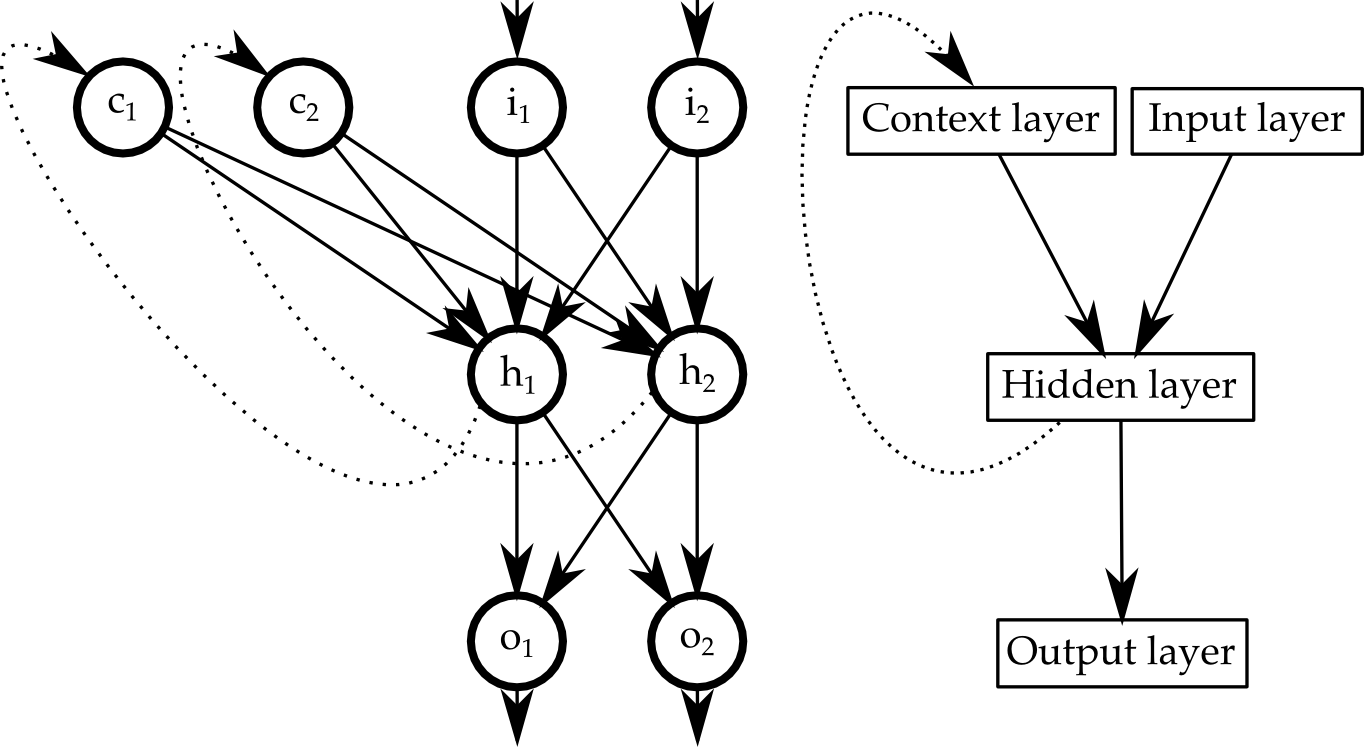
\includegraphics[width=341px]{elman-rnn.png}
		\caption{On the left, Elman's recurrent network with input, hidden, context, and output layer, each containing two units. On the right, schema of layers in Elman network. Dotted link signifies copying activity of source units to target units.}
	\end{figure}

Recurrent network's output in time $t$ is computed in four steps:
\begin{enumerate}
	\item Input vector is copied to activation of input layer units
	\item Activation of hidden layer units in time $t-1$ is copied to current activation of context layer units
	\item Hidden layer units compute their activations
	\item Output layer units compute their activations and copy them to network's output
\end{enumerate}
	
\subsection{Backpropagation Through Time}
Standard backpropagation algorithm is not suited for networks with cycles in them. Fortunately, RNN can be modified to look like a feedforward network by unfolding the network in time as shown in figure \ref{unfolding} and then trained by Backpropagation Through Time (BPTT) algorithm first laid out by Rumelhart, Hinton and Williams \cite{rumelhart-hinton-williams}.\par

The network unfolding process begins with a SRN in current time step $t$, denoted as $SRN_t$. Since context layer of a SRN is just a copy of hidden layer activation from previous step, cycles in the network can be avoided by replacing context layer with an identical copy of the SRN network from previous step, $SRN_{t-1}$. Hidden layer of $SRN_{t-1}$ is then connected to hidden layer of $SRN_t$. This procedure is repeated until time step $0$ is reached, in which case the context layer is not replaced, but rather stays set to its initial activity. The number of SRN copies represents depth of the unfolded network and each copy of the network uses the same set of connection weights.\par

	\begin{figure}[ht]
		\centering
		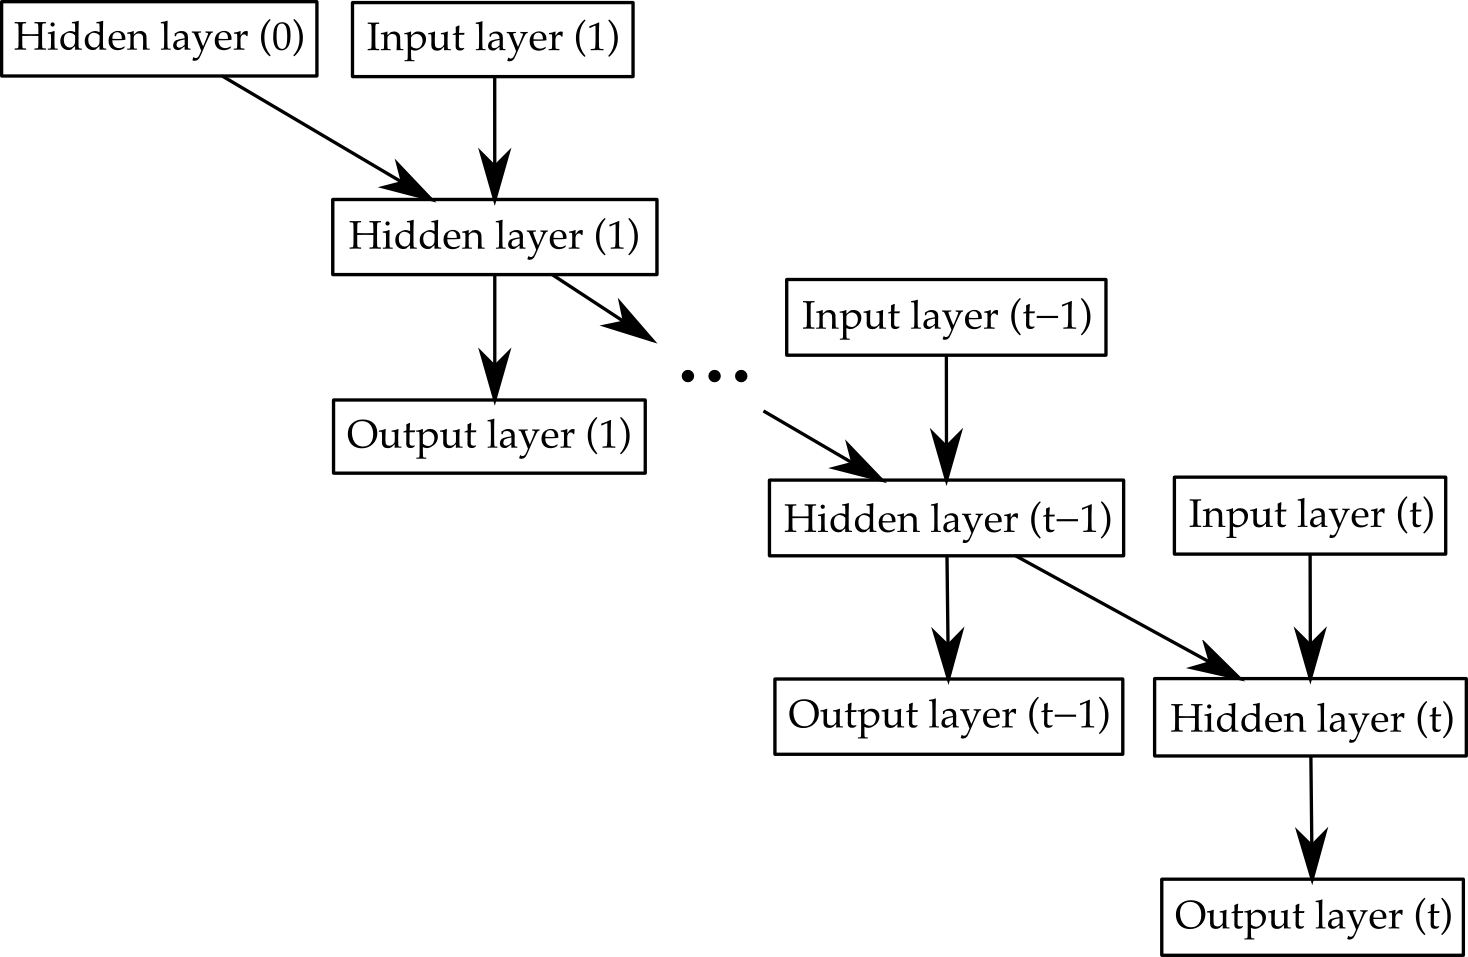
\includegraphics[width=367px]{bptt2.png}
		\caption{Elman's recurrent network unfolded in time. }
		\label{unfolding}
		\label{fig:bptt}
	\end{figure}

Once the SRN has been unfolded into a feedforward network, backpropagation can be used. The algorithm again consists of 3 steps:
\begin{enumerate}
  \item \textbf{Forward propagation}. Signal is propagated through the unfolded network in the standard fashion, from top to bottom. In this case, from the SRN copy furthest in the past to the most recent copy.
  \item \textbf{Backward propagation}. Error term $\Delta^{out}_{i}(t)$ of output layer unit $i$ from SRN copy in time $t$ is computed as
 
  $$\Delta^{out}_{i}(t) = \left(target_{i}(t) - a^{out}_{i}(t)\right) {{\partial{act\left(a^{out}_{i}(t)\right)}} \over {\partial a^{out}_{i}(t)}}$$
 where $target_i(t)$ is desired output of output layer unit $i$ of the SRN in time $t$ and $a^{out}_{i}(t)$ is its actual activation in time $t$.
 
  For every hidden layer unit $i$ of unfolded SRN in time step $t$, let $j$ iterate over all units that receive connections from unit $i$ according to unfolded network topology and let $\Delta_j$ be their error terms. Weight matrix $w_{ij}^h$ holds weights of connections from unit $i$ to unit $j$. Error term of hidden unit $i$ denoted as $\Delta^{hid}_{i}(t)$ is then computed as

  $$\Delta^{hid}_{i}(t) =\left(\sum\limits_{j} \Delta_{j}w_{in}^{h}\right) {{\partial{act\left(a^{hid}_{i}(t)\right)}} \over {\partial a^{hid}_{i}(t)}}$$
  
  \item \textbf{Weights update} in the original SRN. For every unit $j$ in hidden or output layer $l$ of the original network that receives connections from units $i$ in layer $k$, update the weight according to
  %finish this
  $$new \; w_{ij}^l = w_{ij}^l + \alpha \sum\limits_{\tau=0}^{t} \Delta_i^{k}\left(\tau\right) a_{j}^{l}\left(\tau\right)$$
where $w_{ij}^l$ is weight matrix of connections from unit $i$ to unit $j$ in layer $l$, $\Delta_i^{k}(\tau)$ is error term of unit $i$ in layer $k$ of unfolded network copy in time step $\tau$, $a_{j}^{l}(\tau)$ is activation of unit $j$ in layer $l$ of unfolded network copy in time $\tau$ and $\alpha$ is learning rate. One can also add momentum rate analogously to backpropagation described in section \ref{bp}.
\end{enumerate}

\subsection{Truncated Backpropagation Through Time}

In BPTT, Number of SRN copies in the unfolded network is equal to current time step $t$. Should this algorithm be used in online manner, it would be impractical, since its memory footprint grows linearly with time. To overcome this, online version of the BPTT algorithm called Truncated Backpropagation Through Time (TBTT) can be used  \cite{Williams90anefficient}. \par
TBPTT works analogously to BPTT, except the maximum depth $d$ of the unfolded network is limited. Networks are unfolded from current time step $t$ up until $t-d+1$ when unfolding stops. Context layer of the SRN copy in time $t-d-1$ holds activation of network's hidden layer in time $t-d$.\par
TBPTT typically performs backward pass in the unfolded network either every $d$ time steps or at each time step. The latter is examined in this thesis. Since weights of connections are changed every time step, it is appropriate to either store past weights or use current weights but perform a forward propagation pass in the unfolded network.

\subsection{Real-Time Recurrent Learning}
Real-Time Recurrent Learning (RTRL) algorithm is a gradient descent method suitable for online learning of recurrent networks \cite{williams-zipser}.\par

Let there be a SRN whose each unit $i$ has in time step $t$ potential $p_i(t)$ and activation $a_i(t)$. For convenience, let $U_{in}$, $U_{hid}$ and $U_{out}$ be sets of indices of input, hidden and output units respectively. Weight of connection from unit $i$ to unit $j$ is denoted by $w_{ij}$. In time step $t$, let $target_i(t)$ be the teacher given desired activation of output unit $i$.\par

In time step $t$, instantaneous error $E(t)$ is
$$E(t) = {1 \over 2}\sum\limits_{i \in U_{out}}\left(target_i(t) - a_i(t)\right)^2$$
and the minimised total error $E_{total}(t)$ in time $t$  is
$$E_{total}(t) =\sum\limits_{\tau=1}^t E(\tau)$$
The error is minimised by adjusting weights along the negative gradient of error $-\partial E_{total}(t) / \partial w_{ij}$. This can be computed by accumulating negative gradient of instant error in each time step
$$-{{\partial E(t)} \over {\partial w_{ij}}} = \sum\limits_{i \in U_{out}} \left( target_i(t) - a_i(t) \right) {{\partial a_i(t)} \over {\partial w_{ij}}}$$
${\partial a_i(t)} / {\partial w_{ij}}$ can be computed by differentiating the network dynamics equation, resulting in the derivative $v^k_{ij}(t)$ of hidden or output\footnote{Activations of input units do not depend on networks' weights.} unit $k$ activation w.r.t. every weight $w_{ij}$ in time $t$
$$ v^k_{ij}(t+1) = {{\partial a_k(t+1)} \over {\partial w_{ij}}} = act'(p_k(t)) \left[ \left(\sum\limits_{l \in U_{hid} \cup U_{out}}  w_{lk}  v_{ij}^l(t)\right) + \delta_{ki} a_j(t) \right] $$
where $\delta_{ki}$ is Kronecker's delta
$$\delta_{ki} =
    \begin{cases}
            1, &         \text{if } k=i,\\
            0, &         \text{if } k\neq i.
    \end{cases}$$
This creates dynamical system with variables $v^k_{ij}$ for all hidden and output units. Since the initial state of the network is independent from its weights, initial value can be set $v^k_{ij}(0) = 0$. Network's weights are then updated along the accumulated trajectory
$$new \; w_{ij} =  w_{ij} - \alpha \sum\limits_{k \in U_{out}} \left[ \left(a_k(t) - target_k(t) \right) v_{ij}^k \right]$$
One can also add momentum rate analogously to backpropagation described in section \ref{bp}. \par

RTRL algorithm is computationally expensive \cite{minds-jacobs}, because calculating $v^k_{ij}(t+1)$ requires $O(n^4)$ operations, where $n$ is number of hidden and output units. This limits its usage to very small networks.

\section{Clockwork Recurrent Network}
%add citations
SRNs have trouble capturing capturing long-term dependencies in input sequences due to vanishing gradient problem \cite{Hochreiter01gradientflow}. Clockwork recurrent neural network (CW-RNN) is a modification of Elman's SRN architecture designed to solve this problem by having hidden layer split into $M$ modules running at different clocks \cite{cw-rnn}.
Each module $i$ is assigned a clock rate $T_i$. In time step $t$ only modules with clock rate that satisfies $(t \; mod \; T_i) = 0$ compute their activations, other modules retain their previous activation.  \par

Like in SRN, input layer is connected to hidden layer, context layer stores activation of hidden layer from previous time step and hidden layer is connected to output layer. The difference is that module of hidden layer with clock rate $T_i$ connects to module in context layer with period $T_j$ only if $T_i <= T_j$ as shown in figure \ref{cwrnn}.
	\begin{figure}[ht]
		\centering
		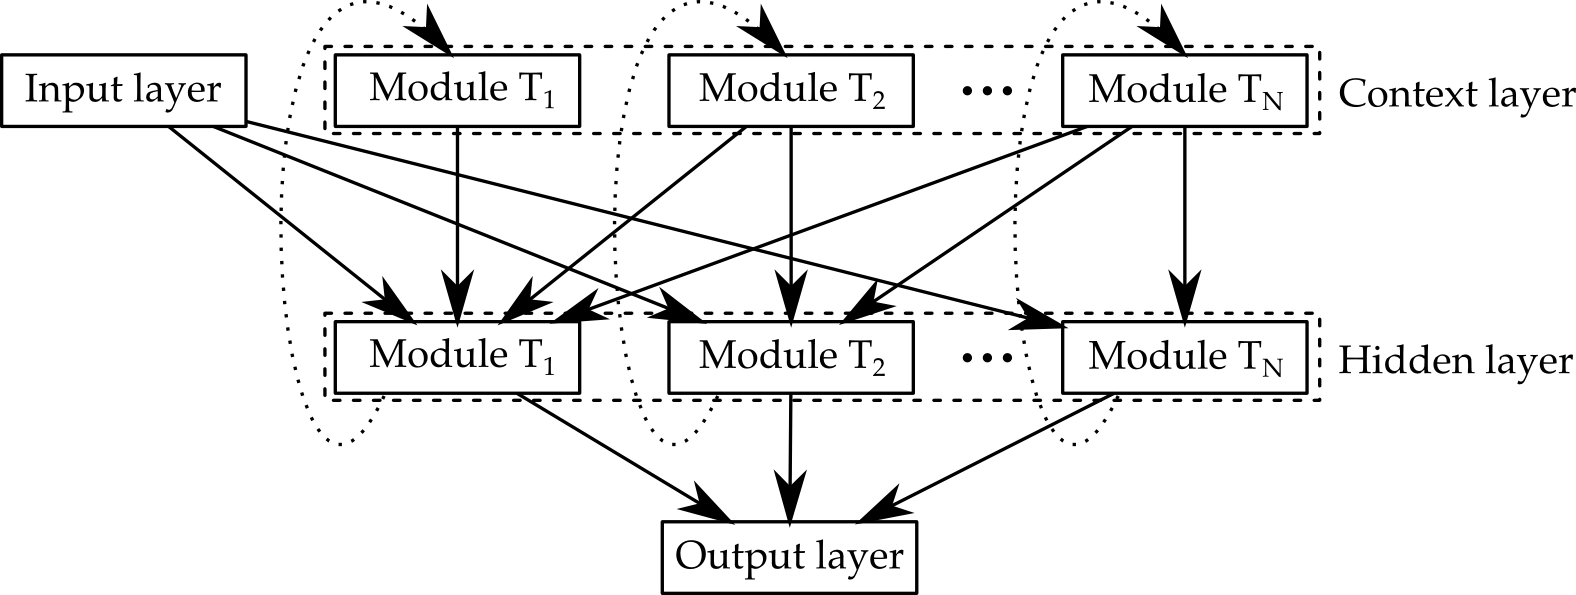
\includegraphics[width=394px]{cw-rnn.png}
		\caption{Clockwork-RNN. }
		\label{cwrnn}
	\end{figure}
This allows slower modules to focus on long-term dependencies in the input sequence, while faster modules focus on short-term information with context provided by slower modules. \par

To adapt network weights, BPTT learning algorithm can be used. The algorithm works analogously with the only difference compared to SRN being that error propagates backwards only from active modules executed at time $t$. Error term of inactive modules is retained from previous step. \par
Since a CW-RNN\footnote{CW-RNN with at least two modules running at different clock rates.} with the same number of units as a SRN has fewer connections and activations of hidden units are computed less frequently, CW-RNN should run faster than SRN with the same number of either weights or units.
      
\chapter{Implementation}
\section{Neural Prediction Library}
As a part of this thesis, Neural Prediction Library (NPL) is built for experimenting with various neural network models in online time series prediction tasks. NPL supports all tested neural network architectures as well as learning algorithms. In addition to that, the tool allows easy manipulation with data points and datasets. NPL is written in C++ programming language and is structured into classes dealing with data manipulation and neural networks.
\subsection{Data Manipulation}
	Data point in NPL is represented using a \textbf{MemoryBlock} object, which encapsulates an array of floating point numbers and provides convenience methods and arithmetic vector operations.\par
	\textbf{DataSet} class enables offline training of the networks by reading data points from a file, where each data point is on a separate line and its values are separated by spaces. \par
	\textbf{DstatParser} class allows reading raw output produced by Dstat tool and converting it to data point format suitable for prediction.
\subsection{Neural Networks}
All implemented neural networks provide the same interface described by abstract class \textbf{NeuralNetwork} consisting of forward propagation of input and retrieval of output. \par
Neural networks are composed of layers implemented by \textbf{NeuralLayer} class which holds activations of its units and weights of incoming connection and on top of that supports forward propagation of input signal and backward propagation of errors using standard backpropagation algorithm. \par
\textbf{FeedforwardNetwork} implements an MLP with variable number of hidden layers and units in them. The topology of the network can be further modified beyond MLP if required. \par
\textbf{CWRecurrentNetwork} implements a CW-RNN with a variable number of hidden layer modules with specified clock rates. \par
\textbf{SimpleRecurrentNetwork} derives from CWRecurrentNetwork to implement a SRN, since Elman's SRN is just a special case of CW-RNN network with single hidden layer module with clock rate equal one. \par

\subsection{Learning Algorithms}
\textbf{LearningAlgorithm} is an abstract class providing common interface for all learning algorithms prescribing a method to train the network with teacher given target and reading current square error. \par
\textbf{Backpropagation, TBPTT, RTRL} classes are descendants of LearningAlgorithm implementing respectively named algorithms. Backpropagation class is used for training a FeedforwardNetwork, RTRL for training a SimpleRecurrentNetwork. TBPTT supports training both SimpleRecurrentNetwork and CWRecurrentNetwork.

\section{Network Monitor}
Network monitor is an application built on top of NPL that works with assistance of UNIX system resources monitoring tool Dstat \cite{dstat}. Dstat provides real-time measurements of system resources and displays them in a format of table that grows by one row each second. Columns of this table represent various measured variables and can be specified with command line options. This interval between measurements can be modified with command line options as well. \par

\begin{figure}[H]
	\centering
	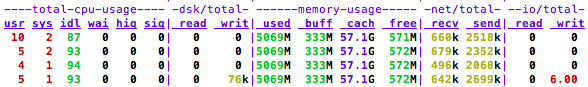
\includegraphics[width=360px]{dstat_sample.png}
	\caption{Sample output from Dstat.}
\end{figure}

Output of Dstat is redirected to the network monitoring program. Raw Dstat output is automatically parsed and preprocessed to serve as input for a neural network of choice. As a proof of concept, the network is constantly predicting incoming and outgoing network traffic and training to improve its precision. Should the difference between prediction and actual value exceed predefined threshold, this incident is logged to a file as an anomaly. Please refer to the $README.txt$ file for instructions on how to launch and use the network monitor.\par


\section{Robotic Arm Simulator}
Robotic arm simulator application is implemented in BEPUPhysics 3D physics library \cite{bepuphysics}. Manipulator with three degrees of freedom from BEPU robotic arm demo \cite{bepu-robotarm-demo} is constructed in 3D world. Three controlled joints are situated in base, "shoulder" and "elbow" of the arm and rotate in one axis.\par

	\begin{figure}[ht]
		\centering
		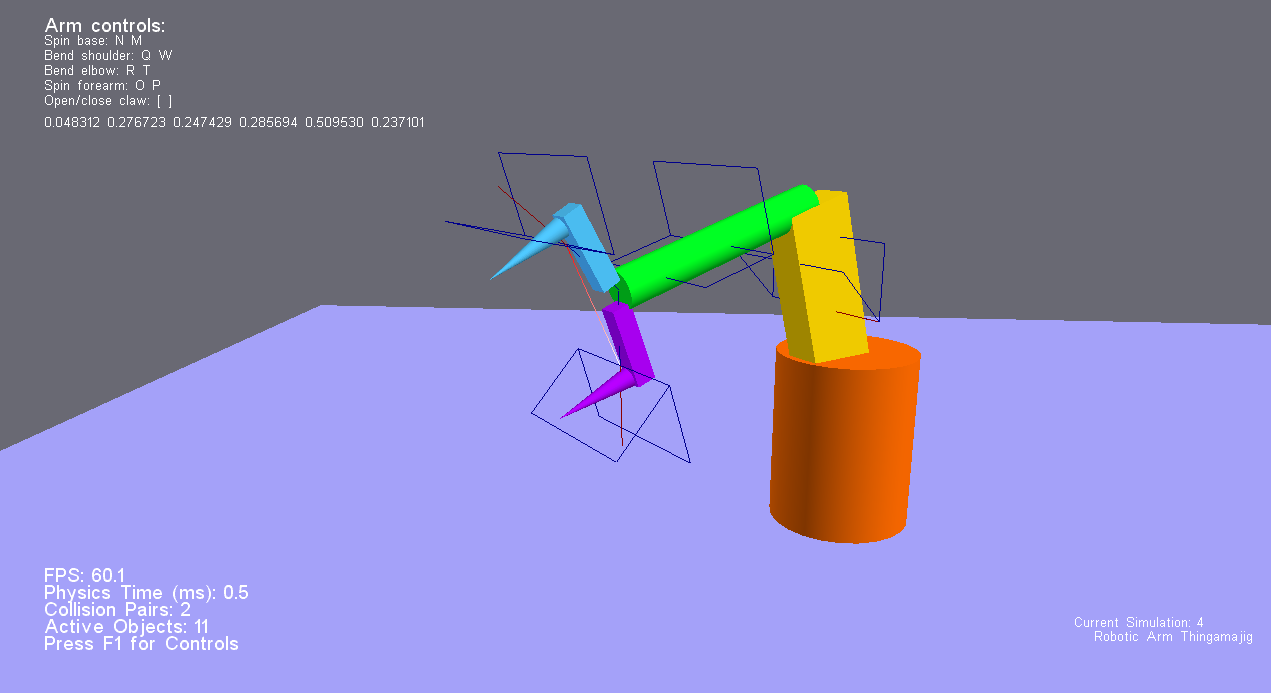
\includegraphics[width=360px]{roboticarm.png}
		\caption{Robotic arm in BEPUPhysics 3D physics simulator.}
	\end{figure}

Simulator renders the scene, calculates physics and supplies information about current rotation of joints as well as position of claw to a neural network of choice, which provides prediction of claw position in next time step. The prediction network thus creates a forward model of the process, in this case a robotic arm, which can find its use in control system, such as Internal Model Control \cite{internal-model-control}. \par
NPL is linked and integrated with the robotic arm simulator. As a proof of concept, line showing direction from current position of claw to the predicted position is drawn. For instructions on how to launch and use the robotic simulator, please refer to the $README.txt$ file.

\chapter{Experiments}
In the following experiments, I attempt to find the best performing network and its hyper parameters for prediction in three different scenarios with restricted computation time.\par

Networks are tested on the same prepared datasets to ensure equal testing conditions. Units of all networks use logistic activation function. Weights of connections in all networks are initialised randomly with uniform distribution on interval [-0.25, 0.25]. Since the initial setting of network influences its overall performance, all experiments described below are run ten times and only the average of them is presented as the result.\par

Experiments measuring computation time are run on 1.7GHz Intel Core i5 2557M. While the absolute computation times should vary depending on system configuration, I expect them to retain their ratio relative to each other. Computation time is measured from the moment just before first data point is processed until the last one is processed.\par

As a measure of prediction accuracy, total error $E_{total}$ collected over $T$ time steps is used. Network that predicts entire sequence flawlessly would have zero total error. %mention higher worse?
$$E_{total} = \sum\limits_{\tau = 1}^T {1 \over 2} \sum\limits_{i=1}^{N}\left(Target_i - Output_i\right)^2$$
Networks are trained online in every time step. In order to capture both their accuracy and ability to adapt quickly, there is no traditional division into training and testing period. Instead, networks are evaluated online as they learn in all time steps. \par

\section{Testing Scenarios}
Networks are tested on three different datasets with varying complexity collected from three scenarios. Each scenario is designed to test a specific aspect of prediction, such as modelling generative processes, noisy network traffic or substantially time constrained robotic manipulator.

\subsection{Goniometric function}
The first simple testing scenario is predicting next step of a generative process with no inputs whose output vector of length one is defined in time $t$ as
$$Output_t ={{1 + sin(t)cos(2t)} \over 2}$$

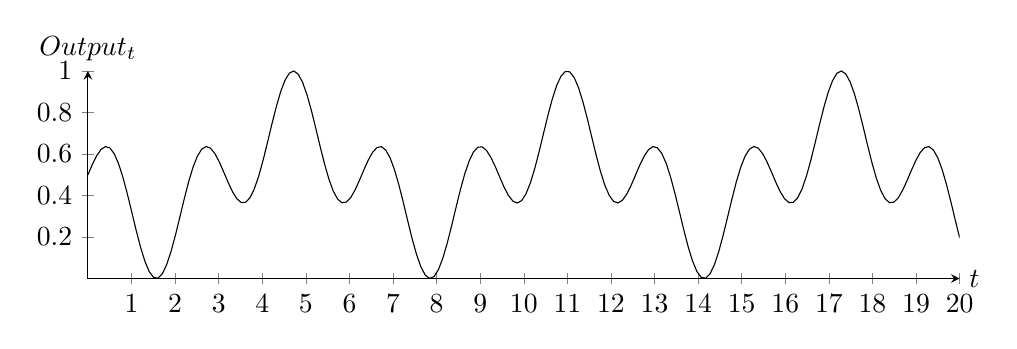
\begin{tikzpicture}[domain=0:20,samples=200]
\begin{axis}[
  axis x line=middle,
  axis y line=middle,
  xmin=0, xmax=20,
  ymin=0, ymax=1,
  height=120,
  width=360,
  xtick={0,1,...,20},
  ytick={0,0.2,...,1},
  xlabel={$t$},
  ylabel={$Output_t$},
  xlabel style={right},
  ylabel style={above},
]
\addplot[]{0.5 + 0.5*sin(deg(x))*cos(deg(2*x))};
\end{axis}
\end{tikzpicture}

The goniometric function's range is [0,1] which matches logistic activation function's range [0,1], therefore no preprocessing is needed. This function is periodical with period of $2\pi$. \par
In time step $t$, a TDNN with sliding window of size $w$ receives input consisting of $Output_{\tau}$ in time steps $\tau$ from $t-w+1$ to $t$ and is tasked to predict $Output_{t+1}$. Similarly, RNNs are tasked to predict $Output_{t+1}$, but they only receive $Output_t$ on their inputs.

\subsection{Network Usage}
Second testing scenario is predicting computer network usage measured by monitoring tool Dstat. Each second, Dstat measures usage of system resources such as CPU load, memory usage, disk throughput, number of open sockets as well as network incoming and outgoing traffic. Prediction has to be computed in less time than it takes Dstat to collect network usage, which poses a loose time constraint of computation time being less than one second. Dataset consists of 3,600 data points created by monitoring real application server for one hour with enabled cpu, disk, memory, network, I/O and socket stats command line options. \par

Dstat measures 26 variables of the monitored system, two of which are incoming and outgoing network traffic. Values of these two variables in next time step shall be predicted. Since the values observed by Dstat have huge dynamic range, preprocessing is necessary. Values are linearly squashed into interval [0, 1] by dividing the observed value by the expected maximum. \par
In time step $t$, a TDNN with sliding window of size $w$ receives input consisting of the 26 measured variables in time steps $\tau$ from $t-w+1$ to $t$ and is tasked to predict two variables --- incoming and outgoing traffic in time step$t+1$. Similarly, RNNs are tasked to predict the same two values, but they only receive the 26 measured variables in time step $t$.


\subsection{Robotic Arm}
Third testing scenario is predicting position of robotic arm's claw in BEPUPhysics 3D physics library. Manipulator with three controlled joints is constructed. At each simulation step, network receives rotations of all three joints and their respective control signals. The goal is to predict next X, Y and Z position of the claw in next time step. The data points are squashed into interval [0,1] by the simulator so they don't require preprocessing.\par
This task is heavily time constrained. The 3D simulator is required to run at 60 frames per second for smooth control, which leaves only $1 \over 60$ of a second for computing the prediction. Dataset consisting of 18,000 data points is created by controlling the robot with random commands for a period of five minutes. \par
In time step $t$, a TDNN with sliding window of size $w$ receives input consisting of X, Y and Z position of the claw, three angles of joints and their three control signals in time steps $\tau$ from $t-w+1$ to $t$ and is tasked to predict claw's X, Y and Z position in time step $t+1$. Similarly, RNNs are tasked to predict the same X, Y and Z position, but they only receive the three joint angles and their three control signals in time step $t$.

\section{Tested Methods}

\subsection{Time Delay Neural Network}
The role of sliding window size is examined w.r.t. prediction accuracy and computation time. TDNNs with a single hidden layer consisting of 64, 128 and 256 units are examined. Learning and momentum rates are informally chosen to the best performing value for each dataset according to the following table.

\begin{table}[h]
\centering
\begin{tabular}{|l|c|c|}
\hline
\multicolumn{1}{|c|}{\textbf{Scenario}} & \textbf{Learning rate} & \textbf{Momentum rate} \\ \hline
Goniometric function                    & 0.05                   & 0.9                    \\ \hline
Network usage                           & 0.001                  & 0.9                    \\ \hline
Robotic arm simulator                   & 0.01                   & 0.9                    \\ \hline
\end{tabular}
\caption{Learning and momentum rates of TDNN in the experiments.}
\end{table}


\subsection{SRN trained by TBPTT}
SRNs with 64, 128 and 256 hidden units trained using TBPTT are tested with varying unfolding depth in order to find its impact on precision and computation time.

\begin{table}[h]
\centering
\begin{tabular}{|l|c|c|}
\hline
\multicolumn{1}{|c|}{\textbf{Scenario}} & \textbf{Learning rate} & \textbf{Momentum rate} \\ \hline
Goniometric function                    & 0.01                   & 0.99                    \\ \hline
Network usage                           & 0.001                  & 0.9                    \\ \hline
Robotic arm simulator                   & 0.01                   & 0.9                    \\ \hline
\end{tabular}
\caption{Learning and momentum rates  of SRN trained by BPTT in the experiments.}
\end{table}


\subsection{SRN trained by RTRL}
Due to RTRL's severe computational complexity, SRNs with only 8 and 16 hidden units are tested for prediction accuracy and computation time. In all scenarios, learning rate is set to 0.1 and momentum to 0.9.

\subsection{CW-RNN trained by TBPTT}
Experiments examine role of unfolding depth in CW-RNN with 64, 128 and 256 hidden units on its precision and computation time. Hidden layer of the network is divided into four equally big modules with exponential clock rates: 1, 2, 4 and 8.

\begin{table}[h]
\centering
\begin{tabular}{|l|c|c|}
\hline
\multicolumn{1}{|c|}{\textbf{Scenario}} & \textbf{Learning rate} & \textbf{Momentum rate} \\ \hline
Goniometric function                    & 0.01                   & 0.99                    \\ \hline
Network usage                           & 0.001                  & 0.9                    \\ \hline
Robotic arm simulator                   & 0.01                   & 0.9                    \\ \hline
\end{tabular}
\caption{Learning and momentum rates of CW-RNN trained by BPTT in the experiments.}
\end{table}

\chapter{Results}
\section{Goniometric Function Results}
\subsection{Role of TDNN's Sliding Window Size}
The results show steep decrease of error when increasing window size from two to three past time steps and mild decrease of error when extending window further. Presumably, three steps are threshold when information in the sliding window becomes sufficient to capture dynamics of the simple goniometric function. Network with only 64 hidden units performed notably worse than bigger networks. However, there is no significant gain in increasing network size beyond 128 hidden units.

	\begin{figure}[H]
		\caption{Total error of predicting goniometric function with TDNN and various sliding window sizes.}
		\centering
\begin{tikzpicture}
	\begin{axis}[
	  xlabel=Sliding window size,
	  ylabel=Total error,
	  xmin = 0,
	  ymin = 0,
	  axis lines = left,
	  xtick={1,2,...,20},
 	  ytick={0,10,...,60},
	  legend pos=north east,
	  height=130,
	  width=360]
 	\addplot table [x=WS, y=ERROR64]{results/tdnn_gon.dat};
	\addlegendentry{64 hidden units}
	\addplot table [x=WS, y=ERROR128]{results/tdnn_gon.dat};
	\addlegendentry{128 hidden units}
	\addplot table [x=WS, y=ERROR256]{results/tdnn_gon.dat};
	\addlegendentry{256 hidden units}
	\end{axis}
\end{tikzpicture}
	\end{figure}


\subsection{Role of TBPTT Unfolding Depth}
In both SRN and CW-RNN, increasing unfolding depth decreases total prediction error. Increasing hidden layer size helps both networks find better error minimum. In this scenario, SRN provides better results than CW-RNN with the same hidden layer size.

	\begin{figure}[H]
		\caption{Total error of predicting goniometric function with SRN trained by TBPTT with various unfolding depth.}
		\centering
\begin{tikzpicture}
	\begin{axis}[
	  xlabel=Unfolding depth,
	  ylabel=Total error,
	  xmin = 0,
	  ymin = 0,
	  axis lines = left,
	  xtick={1,2,...,20},
 	  ytick={0,10,...,60},
	  legend pos=south west,
	  height=130,
	  width=360]
	\addplot table [x=UD, y=ERROR64]{results/tbptt_gon.dat};
	\addlegendentry{64 hidden units}
	\addplot table [x=UD, y=ERROR128]{results/tbptt_gon.dat};
	\addlegendentry{128 hidden units}
	\addplot table [x=UD, y=ERROR256]{results/tbptt_gon.dat};
	\addlegendentry{256 hidden units}
	\end{axis}
\end{tikzpicture}

		
		\caption{Total error of predicting goniometric function with CW-RNN trained by TBPTT with various unfolding depth.}
		\centering
\begin{tikzpicture}
	\begin{axis}[
	  xlabel=Unfolding depth,
	  ylabel=Total error,
	  xmin = 0,
	  ymin = 0,
	  axis lines = left,
	  xtick={1,2,...,20},
 	  ytick={0,10,...,60},
	  legend pos=south west,
	  height=130,
	  width=360]
	\addplot table [x=UD, y=ERROR64]{results/cw_gon.dat};
	\addlegendentry{64 hidden units}
	\addplot table [x=UD, y=ERROR128]{results/cw_gon.dat};
	\addlegendentry{128 hidden units}
	\addplot table [x=UD, y=ERROR256]{results/cw_gon.dat};
	\addlegendentry{256 hidden units}
	\end{axis}
\end{tikzpicture}

	\end{figure}

\subsection{Computation Time Tradeoff}
The most accurate network in predicting goniometric function was TDNN with 128 hidden units and sliding window of 20 past steps. In this simple task, TDNN shows remarkable performance while also being the least computationally extensive. \par
SRN trained by TBPTT achieves the second best result, though with much higher computation time. While CW-RNN requires approximately only a half of SRN's computation time with the same network size and unfolding depth, in this scenario SRN offers lower error per computation time.\par
SRN trained by RTRL didn't perform particularly well, primarily because of its high computation complexity which limits the maximum practical network size to 32 units.\par
In the following figure, all four methods are compared at how decreasing total error affects computation time. Depicted below are TDNN with 128 hidden units and various sliding window sizes, SRN and CW-RNN with 256 hidden units trained by TBPTT with various unfolding depth, and SRN trained by RTRL with 8, 16 and 32 hidden units.

	\begin{figure}[H]
		\caption{Tradeoff between time and error in goniometric function scenario.}
		\centering
\begin{tikzpicture}
	\begin{axis}[
	  xlabel=Computation time (s),
	  ylabel=Total error,
	  xmin = 0,
	  %xmax=6,
	  ymin = 0,
	  axis lines = left,
%	  xtick={1,2,...,20},
%	  ytick={0,10,...,60},
	  legend pos=north east,
	  height=190,
	  width=360]

	\addplot table [x=TIME128, y=ERROR256]{results/tdnn_gon.dat};
	\addlegendentry{TDNN}

	\addplot table [x=TIME256, y=ERROR256]{results/tbptt_gon.dat};
	\addlegendentry{TBPTT}
	
	\addplot table [x=TIME256, y=ERROR256]{results/cw_gon.dat};
	\addlegendentry{CW-RNN}

	\addplot table [x=TIMEG, y=ERRORG]{results/rtrl.dat};
	\addlegendentry{RTRL}
	\end{axis}
\end{tikzpicture}

	\end{figure}

\section{Network Usage Results}
Number of hidden units, sliding window size and unfolding depth show little effect on reducing total error. This behaviour could be caused by inherent unpredictability of the network traffic or inability of the methods to find the correct model.\par
The best performing method was RTRL with 16 hidden units closely followed by TDNN.

	\begin{figure}[H]
		\caption{Total error of predicting network traffic with TDNN and various sliding window sizes.}
		\centering
\begin{tikzpicture}
	\begin{axis}[
	  xlabel=Sliding window size,
	  ylabel=Total error,
	  xmin = 0,
	  ymin = 0,
	  ymax=65,
	  axis lines = left,
%	  xtick={1,2,...,20},
%	  ytick={0,10,...,70},
	  legend pos=south east,
	  height=160,
	  width=360]
	 \addplot table [x=WS, y=ERROR64]{results/tdnn_net.dat};
	\addlegendentry{64 hidden units}
	\addplot table [x=WS, y=ERROR128]{results/tdnn_net.dat};
	\addlegendentry{128 hidden units}
	\addplot table [x=WS, y=ERROR256]{results/tdnn_net.dat};
	\addlegendentry{256 hidden units}
	\end{axis}
\end{tikzpicture}


		\caption{Total error of predicting network traffic with SRN trained by TBPTT with various unfolding depth.}
		\centering
\begin{tikzpicture}
	\begin{axis}[
	  xlabel=Unfolding depth,
	  ylabel=Total error,
	  xmin = 0,
	  ymin = 0,
	  axis lines = left,
	  xtick={1,2,...,20},
 	  ytick={0,10,...,60},
	  legend pos=south west,
	  height=180,
	  width=360]
	\addplot table [x=UD, y=ERROR64]{results/tbptt_net.dat};
	\addlegendentry{64 hidden units}
	\addplot table [x=UD, y=ERROR128]{results/tbptt_net.dat};
	\addlegendentry{128 hidden units}
	\addplot table [x=UD, y=ERROR256]{results/tbptt_net.dat};
	\addlegendentry{256 hidden units}
	\end{axis}
\end{tikzpicture}


		\caption{Total error of predicting network traffic with CW-RNN trained by TBPTT with various unfolding depth.}
		\centering
\begin{tikzpicture}
	\begin{axis}[
	  xlabel=Unfolding depth,
	  ylabel=Total error,
	  xmin = 0,
	  ymin = 0,
	  axis lines = left,
	  xtick={1,2,...,20},
 	  ytick={0,10,...,60},
	  legend pos=south west,
	  height=140,
	  width=360]
	\addplot table [x=UD, y=ERROR64]{results/cw_net.dat};
	\addlegendentry{64 hidden units}
	\addplot table [x=UD, y=ERROR128]{results/cw_net.dat};
	\addlegendentry{128 hidden units}
	\addplot table [x=UD, y=ERROR256]{results/cw_net.dat};
	\addlegendentry{256 hidden units}
	\end{axis}
\end{tikzpicture}

	\end{figure}

\subsection{Computation Time Tradeoff}
No tested model exceeded the maximum allowed computation time of one hour. Small networks trained by RTRL perform well and maintain viable computation time. TDNN achieved the second lowest precision while using the least computation time. Networks trained by TBPTT achieve better results with smaller unfolding depth.\par
In the following figure, SRN with 8, 16 and 32 hidden units trained by RTRL is compared to other models with 256 units.
	\begin{figure}[H]
		\caption{Tradeoff between time and error in network usage scenario.}
		\centering
\begin{tikzpicture}
	\begin{axis}[
	  xlabel=Computation time (s),
	  ylabel=Total error,
	  xmin = 0,
	  %xmax=6,
	  ymin = 0,
	  axis lines = left,
%	  xtick={1,2,...,20},
%	  ytick={0,10,...,60},
	  legend pos=south east,
	  height=190,
	  width=360]

	\addplot table [x=TIME128, y=ERROR128]{results/tdnn_net.dat};
	\addlegendentry{TDNN}

	\addplot table [x=TIME128, y=ERROR128]{results/tbptt_net.dat};
	\addlegendentry{TBPTT}
	
	\addplot table [x=TIME128, y=ERROR128]{results/cw_net.dat};
	\addlegendentry{CW-RNN}

	\addplot table [x=TIMEN, y=ERRORN]{results/rtrl.dat};
	\addlegendentry{RTRL}
	\end{axis}
\end{tikzpicture}

	\end{figure}
	
\section{Robotic Arm Results}
\subsection{Role of TDNN's Sliding Window Size}
Regardless of number of hidden units, TDNNs find their error minimum with window of size two or three. Enlarging the  window further has negative impact and increases error. The larger the network, the more susceptible it is to this phenomenon. This may suggest that the state of manipulator is sufficiently captured in two or three consecutive steps. Increasing the number of hidden units is distinctly decreasing total error.

	\begin{figure}[H]
		\caption{Total error of predicting manipulator's claw position with TDNN and various sliding window sizes.}
		\centering
\begin{tikzpicture}
	\begin{axis}[
	  xlabel=Sliding window size,
	  ylabel=Total error,
	  xmin = 0,
	  ymin = 0,
	  %ymax=65,
	  axis lines = left,
%	  xtick={1,2,...,20},
	  ytick={0,10,...,120},
	  legend pos=south east,
	  height=160,
	  width=360]
  	\addplot table [x=WS, y=ERROR64]{results/tdnn_man.dat};
	\addlegendentry{64 hidden units}
	\addplot table [x=WS, y=ERROR128]{results/tdnn_man.dat};
	\addlegendentry{128 hidden units}
	\addplot table [x=WS, y=ERROR256]{results/tdnn_man.dat};
	\addlegendentry{256 hidden units}
	\end{axis}
\end{tikzpicture}		
	\end{figure}
	
\subsection{Role of TBPTT Unfolding Depth}
As unfolding depth increases, both SRN and CW-RNN show similar pattern of first sharply decreasing the total error, finding their minimum, and then error gradually rises. Networks with more hidden units perform better in this scenario.

	\begin{figure}[H]
		\caption{Total error of predicting manipulator's claw position with SRN trained by TBPTT with various unfolding depth.}
		\centering
\begin{tikzpicture}
	\begin{axis}[
	  xlabel=Unfolding depth,
	  ylabel=Total error,
	  xmin = 0,
	  ymin = 0,
	  axis lines = left,
	  xtick={1,2,...,20},
 	  ytick={0,25,...,220},
	  legend pos=north east,
	  height=180,
	  width=360]
	\addplot table [x=UD, y=ERROR64]{results/tbptt_man.dat};
	\addlegendentry{64 hidden units}
	\addplot table [x=UD, y=ERROR128]{results/tbptt_man.dat};
	\addlegendentry{128 hidden units}
	\addplot table [x=UD, y=ERROR256]{results/tbptt_man.dat};
	\addlegendentry{256 hidden units}
	\end{axis}
\end{tikzpicture}

	\end{figure}
	
	\begin{figure}[H]	
		\caption{Total error of predicting manipulator's claw position with CW-RNN trained by TBPTT with various unfolding depth.}
		\centering
\begin{tikzpicture}
	\begin{axis}[
	  xlabel=Unfolding depth,
	  ylabel=Total error,
	  xmin = 0,
	  ymin = 0,
	  axis lines = left,
	  xtick={1,2,...,20},
	  ytick={0,25,...,225},
	  legend pos=north east,
	  height=150,
	  width=360]
	\addplot table [x=UD, y=ERROR64]{results/cw_man.dat};
	\addlegendentry{64 hidden units}
	\addplot table [x=UD, y=ERROR128]{results/cw_man.dat};
	\addlegendentry{128 hidden units}
	\addplot table [x=UD, y=ERROR256]{results/cw_man.dat};
	\addlegendentry{256 hidden units}
	\end{axis}
\end{tikzpicture}

	\end{figure}
	
\subsection{Computation Time Tradeoff}
In this heavily time constrained scenario, many neural network models fail to meet the maximum computation time of 300 seconds. RTRL ends up particularly bad on this front, with its network consisting of 32 hidden units using up more than 7 times the maximum computation time. Smaller SRNs trained by RTRL that meet the requirement are not precise enough.\par
TDNN again shows its lightweight computation complexity and beats all networks in this regard, however it scores only third in precision. \par
SRN trained by TBPTT has a slight edge over CW-RNN in precision, but on the other hand, CW-RNN has a much lower computation complexity. Since both methods can fit into required maximum computation time, the final choice of the method should be based on whether one prefers increased precision or lower computation time. \par
In the following figure, TDNN with 256 hidden units and varying sliding window size, SRN and CW-RNN with 256 hidden units trained by TBPTT with varying unfolding depth, and SRN with 8, 16 and 32 hidden units trained by RTRL.

	\begin{figure}[H]
		\caption{Tradeoff between time and error in robotic arm scenario.}
		\centering
\begin{tikzpicture}
	\begin{axis}[
	  xlabel=Computation time (s),
	  ylabel=Total error,
	  xmin = 0,
	  ymin = 0,
	  axis lines = left,
	  xtick={0,250,...,2250},
%	  ytick={0,10,...,60},
	  legend pos=north east,
	  height=180,
	  width=360]

	\addplot table [x=TIME256, y=ERROR256]{results/tdnn_man.dat};
	\addlegendentry{TDNN}

	\addplot table [x=TIME256, y=ERROR256]{results/tbptt_man.dat};
	\addlegendentry{TBPTT}
	
	\addplot table [x=TIME256, y=ERROR256]{results/cw_man.dat};
	\addlegendentry{CW-RNN}
		
	\addplot table [x=TIMEM, y=ERRORM]{results/rtrl.dat};
	\addlegendentry{RTRL}
	
	\end{axis}
\end{tikzpicture}

	\end{figure}

\chapter{Conclusion}
This thesis compared several neural network approaches for online prediction of time series. The examined methods include TDNN, SRN trained by TBPTT and RTRL as well as CW-RNN trained by TBPTT. Role of network size and other parameters w.r.t. prediction accuracy and computation time is evaluated in one synthetic and two real-world datasets. \par
TDNNs have shown to be the least computationally expensive method while providing reasonably good results with appropriately sized sliding window. TBPTT shows consistently good results, albeit with higher computation time. CW-RNN slightly lags behind SRN in precision, but requires less than half of computation time with the same number of units and unfolding depth. RTRL proved to be too impractical to be included in real-world applications where smaller networks aren't sufficient due to its huge computational complexity. Methods struggled the most with predicting computer network usage, most likely due to its inherent unpredictability.\par
As a part of the work, a tool for experimenting with various network architectures and learning algorithms was built and incorporated into two applications. The first is a network monitoring program that detects and logs unexpected events in network traffic. The second application integrates with a robotic simulator to predict position of an arm which may later find its use in control systems.\par
While this thesis examines several methods of predicting time series using neural networks, there are many opportunities to extend it with comparison of other machine learning approaches in the future.


    \appendix
    \chapter{Appendix}
    Source code of all tested models and experiments can be found at https://github.com/karolkuna/Time-Series-Prediction-Using-Neural-Networks\par
    \section{List of attachments}
    \begin{itemize}
    	\item NPL source code with all presented experiments
	\item Network monitor source code
	\item BEPUPhysics solution with incorporated NPL showing prediction of robot's claw
	\item Instructions how to launch and use the mentioned programs
    \end{itemize}
    
    % Bibliography goes here
	\bibliographystyle{plain}
	\bibliography{bibliography}
    
    % Index goes here (optional)
\end{document}











